\documentclass{bredelebeamer}

%%%%%%%%%%%%%%%%%%%%%%%%%%%%%%%%%%%%%%%%%%%%%%%%

\title[Programación en MatLAB]{Introducción a la programación con MatLAB}
\subtitle{Módulo 11 - Matemática simbólica}

\author{- AUTORES -\inst{1}}
\institute[UNIVERSIDAD]
{
  \inst{1}%
  - NOMBRE UNIVERSIDAD -
  }

\date{AÑO}

\subject{Taller de programación}

\logo{

\includegraphics[scale=0.15]{images/logo.png}
}

%%%%%%%%%%%%%%%%%%%%%%%%%%%%%%%%%%%%%%%%%%%%%%%%%%%%%%%%%%%%%%%%%%%%%
\begin{document}

\begin{frame}
  \titlepage 
\end{frame}

%%%%%%%%%%%%%%%%%%%%%%%%%%%%%%%%%%%%%%%%%%%%%%%%%%%%%%%%%%%%%%%%%%%%%

% Álgebra matricial

%%%%%%%%%%%%%%%%%%%%%%%%%%%%%%%%%%%%%%%%%%%%%%%%%%%%%%%%%%%%%%%%%%%%%
\section{Matemática simbólica}

\begin{frame}{Introducción}
\textbf{Objetivos de esta unidad:}




\begin{columns}
\begin{column}{0.35\textwidth}
\begin{center}

\includegraphics[scale=0.4]{images/img40.png}
\end{center}
\end{column}
\begin{column}{0.8\textwidth}
\begin{center}
\begin{itemize}
\item Crear y manipular variables simbólicas
\item Resolver expresiones y ecuaciones simbólicas
\item Graficar ecuaciones simbólicas
\item Introducir a la diferenciación y integración de ecuaciones simbólicas
\end{itemize}
\end{center}
\end{column}
\end{columns}




\end{frame}

\begin{frame}{Creación de variables simbólicas}
\textbf{Declaración de variable simbólica:}
\begin{enumerate}
\item x = sym('x')
\item syms x
\end{enumerate}
\begin{center}
Ambas formas hacen al carácter 'x' igual a la variable simbólica x.
\end{center}
\textbf{Variable simbólica utilizando otras existentes:}
\begin{equation*}
y = \frac{2*(x+3)^2}{x^2+6*x+9}
\end{equation*}
\end{frame}

\begin{frame}{Creación de variables simbólicas}
\textbf{Declaración de variable simbólica:}
\begin{enumerate}
\item x = sym('x')
\item syms x
\end{enumerate}
\begin{center}
Ambas formas hacen al carácter 'x' igual a la variable simbólica x.
\end{center}
\textbf{Variable simbólica utilizando otras existentes:}
\begin{equation*}
y = \frac{2*(x+2)^2}{x^2+6*x+9}
\end{equation*}
\begin{block}{Tener en cuenta}
El comando \textbf{syms} permite crear múltiples variables simbólicas al mismo tiempo.
\end{block}
\end{frame}

\begin{frame}{Creación de variables simbólicas}
\begin{equation*}
syms x
\end{equation*}
\begin{equation*}
y = \frac{2*(x+2)^2}{x^2+6*x+9}
\end{equation*}
\begin{columns}
\begin{column}{0.5\textwidth}
\begin{center}
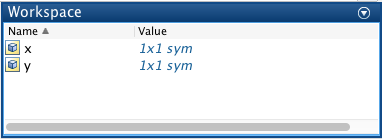
\includegraphics[scale=0.4]{images/fig1.png}
\end{center}
\end{column}
\begin{column}{0.5\textwidth}
\begin{center}
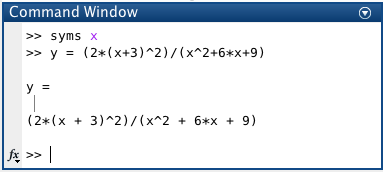
\includegraphics[scale=0.4]{images/fig2.png}
\end{center}
\end{column}
\end{columns}
\end{frame}

\begin{frame}{Manipulación de expresiones y ecuaciones simbólicas}
\textbf{Extracción de numeradores y denominadores:}
\begin{exampleblock}{Comando}
Ver comando: [num,den] = numden(var)
\end{exampleblock}
Ej. Ejecutar las siguientes líneas. Obtener conclusiones.
\lstinputlisting[xleftmargin=.3\textwidth]{scripts/ej1.m}
\end{frame}

\begin{frame}{Manipulación de expresiones y ecuaciones simbólicas}
\textbf{Expansión de expresiones:}
\begin{exampleblock}{Comando}
Ver comando: expand(var)
\end{exampleblock}
Ej. Ejecutar las siguientes líneas. Obtener conclusiones.
\lstinputlisting[xleftmargin=.3\textwidth]{scripts/ej2.m}
\end{frame}

\begin{frame}{Manipulación de expresiones y ecuaciones simbólicas}
\textbf{Factorización de expresiones:}
\begin{exampleblock}{Comando}
Ver comando: factor(var)
\end{exampleblock}
Ej. Ejecutar las siguientes líneas. Obtener conclusiones.
\lstinputlisting[xleftmargin=.3\textwidth]{scripts/ej3.m}
\end{frame}

\begin{frame}{Manipulación de expresiones y ecuaciones simbólicas}
\textbf{Recolección de términos:}
\begin{exampleblock}{Comando}
Ver comando: collect(var)
\end{exampleblock}
Ej. Ejecutar las siguientes líneas. Obtener conclusiones.
\lstinputlisting[xleftmargin=.3\textwidth]{scripts/ej4.m}
\end{frame}

\begin{frame}{Simplificación de ecuaciones simbólicas}
\textbf{Simplificación de ecuación:}
\begin{exampleblock}{Comando}
Ver comando: simplify(var)
\end{exampleblock}
Ej. Ejecutar las siguientes líneas. Obtener conclusiones.
\lstinputlisting[xleftmargin=.3\textwidth]{scripts/ej5.m}
\end{frame}

\begin{frame}{Ejercicio práctico 18}
\begin{enumerate}
\item Cree la variable simbólica x y verifique que se encuentra en el workspace
\item Cree las siguientes expresiones simbólicas:
\begin{itemize}
\item $ex1 = x^2-1$
\item $ex2 = (x+1)^2$
\end{itemize}
\item Multiplique ex1 por ex2 y llame al resultado y1
\item Divida ex1 entre ex2 y llame al resultado y2
\item Use la función \textbf{numden} para extraer el numerador y denominador de y1 y y2
\item Use las funciones \textbf{factor}, \textbf{expand}, \textbf{collect} y \textbf{simplify} en y1 e y2.
\end{enumerate}
\end{frame}

\begin{frame}{Resolución de expresiones y ecuaciones simbólicas}
\textbf{Resolución de expresiones y ecuaciones:}
\begin{exampleblock}{Comando}
Ver comando: solve()
\end{exampleblock}
Se utilizarán dos enfoques, los mismos son:
\begin{enumerate}
\item Cuando se trata de una expresión
\item Cuando se trata de una ecuación
\begin{enumerate}
\item Expresión igualada a 0
\item Expresión igualada a una expresión (aplicando transformación)
\item Expresión igualada a una expresión (sin transformación)
\end{enumerate}
\end{enumerate}
\end{frame}

\begin{frame}{Resolución de expresiones y ecuaciones simbólicas: Caso 1}
\textbf{Utilización de la función solve en una expresión:}\\
Ej. Ejecutar las siguientes líneas. Obtener conclusiones.
\lstinputlisting[xleftmargin=.3\textwidth]{scripts/ej6.m}
\end{frame}

\begin{frame}{Resolución de expresiones y ecuaciones simbólicas: Caso 1}
\textbf{Utilización de la función solve en una expresión:}\\
Ej. Ejecutar las siguientes líneas. Obtener conclusiones.
\lstinputlisting[xleftmargin=.3\textwidth]{scripts/ej6.m}
\begin{alertblock}{Importante}
Cuando se usa en una expresión, la función \textbf{solve} iguala la expresión a cero y resuelve.
\end{alertblock}
\end{frame}

\begin{frame}{Resolución de expresiones y ecuaciones simbólicas: Caso 1}
\textbf{Especificación de la variable a resolver:}\\
Ej. Ejecutar las siguientes líneas. Obtener conclusiones.
\lstinputlisting[xleftmargin=.3\textwidth]{scripts/ej13.m}
\begin{alertblock}{Importante}
Matlab por defecto resuelve para la variable simbólica x. 
\end{alertblock}
\end{frame}

\begin{frame}{Resolución de expresiones y ecuaciones simbólicas: Caso 2.1 ó 2.2}
\textbf{Transformación en una expresión:}\\
Para el caso:
\begin{equation*}
5*x^2+6*x+3=10
\end{equation*}
Se podría reformular como:
\begin{equation*}
5*x^2+6*x-7=0
\end{equation*}
y resolver la ecuación ejecutando las siguientes líneas:
\lstinputlisting[xleftmargin=.3\textwidth]{scripts/ej7.m}
\end{frame}

\begin{frame}{Resolución de expresiones y ecuaciones simbólicas: Caso 2.3}
\textbf{Sin transformación de expresión:}\\
Para el caso:
\begin{equation*}
5*x^2+6*x+3=10
\end{equation*}

Se resuelve la ecuación ejecutando las siguientes líneas:
\lstinputlisting[xleftmargin=.3\textwidth]{scripts/ej8.m}
\end{frame}

\begin{frame}{Ejercicio práctico 19}
\begin{enumerate}
\item Cree las variables simbólicas x,a,b y c 
\item Cree las siguientes expresiones simbólicas:
\begin{itemize}
\item $ex1 = a*x^2-1$
\item $ex2 = a*x^2+b*x+c$
\end{itemize}
\begin{itemize}
\item $eq1 = a*x^2=1$
\item $eq2 = a*x^2+b*x+c=0$
\end{itemize}
\item Use la función solve para resolver ex1 y eq1 tanto para x como para a
\item Use la función solve para resolver ex2 y eq2 tanto para x como para a
\end{enumerate}
\end{frame}

\begin{frame}{Resolución de sistemas de ecuaciones}
\textbf{Resolver el siguiente sistemas de ecuaciones:}
\begin{equation*}
\left\{\begin{matrix}
3x + 2y - z = 10  \\ 
-x +3y +2z = 5  \\ 
 x - y - z = -1 
\end{matrix}\right.
\end{equation*}
\end{frame}

\begin{frame}{Resolución de sistemas de ecuaciones}
\begin{itemize}
\item Definir las tres ecuaciones simbólicas
\end{itemize}
\lstinputlisting[xleftmargin=.3\textwidth]{scripts/ej15.m}
\end{frame}

\begin{frame}{Resolución de sistemas de ecuaciones}
\begin{itemize}
\item Definir las tres ecuaciones simbólicas
\end{itemize}
\lstinputlisting[xleftmargin=.3\textwidth]{scripts/ej15.m}
Luego utilizando la función \textbf{solve} se obtienen la solución (valores de x, y, z):
\lstinputlisting[xleftmargin=.3\textwidth]{scripts/ej14.m}
\end{frame}

\begin{frame}{Graficación de ecuaciones simbólicas}
\textbf{Graficación de y=f(x):}
\begin{exampleblock}{Comando}
Ver comando: ezplot()
\end{exampleblock}
Ej. Ejecutar las siguientes líneas. Obtener conclusiones.
\lstinputlisting[xleftmargin=.3\textwidth]{scripts/ej9.m}
\end{frame}

\begin{frame}{Graficación de ecuaciones simbólicas}
\textbf{Graficación de y=f(x):}
\begin{exampleblock}{Comando}
Ver comando: ezplot()
\end{exampleblock}
Ej. Ejecutar las siguientes líneas. Obtener conclusiones.
\lstinputlisting[xleftmargin=.3\textwidth]{scripts/ej9.m}
\begin{alertblock}{Importante}
Por defecto, se grafica la función con una variación de x en el intervalo $[-2*\pi ,2*\pi ]$
\end{alertblock}
\end{frame}

\begin{frame}{Graficación de ecuaciones simbólicas}
Ej. Ejecutar las siguientes líneas. Obtener conclusiones.
\lstinputlisting[xleftmargin=.3\textwidth]{scripts/ej10.m}
\begin{center}
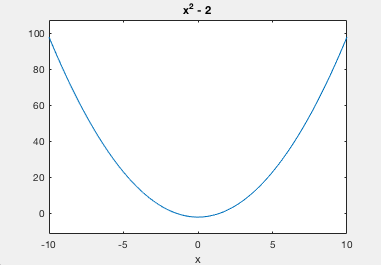
\includegraphics[scale=0.4]{images/fig3.png}
\end{center}
\end{frame}

\begin{frame}{Graficación de ecuaciones simbólicas}
\textbf{Ecuaciones paramétricas:}
\begin{center}
\begin{equation*}
x = sen(t)
\end{equation*}
\begin{equation*}
y = cos(t)
\end{equation*}
\end{center}
Ej. Ejecutar las siguientes líneas. Obtener conclusiones.
\lstinputlisting[xleftmargin=.3\textwidth]{scripts/ej11.m}
\begin{center}
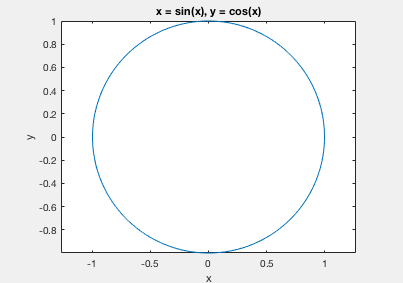
\includegraphics[scale=0.3]{images/fig4.png}
\end{center}
\end{frame}

\begin{frame}{Graficación de ecuaciones simbólicas}
\begin{center}
\begin{equation*}
y1 = sym('sen(X)') 
\end{equation*}
\begin{equation*}
y2 = sym('sen(2*X)') 
\end{equation*}
\begin{equation*}
y3 = sym('sen(3*X)') 
\end{equation*}
\end{center}
Ej. Ejecutar las siguientes líneas. Obtener conclusiones.
\lstinputlisting[xleftmargin=.4\textwidth]{scripts/ej12.m}
\end{frame}

\begin{frame}{Graficación de ecuaciones simbólicas}
\begin{center}
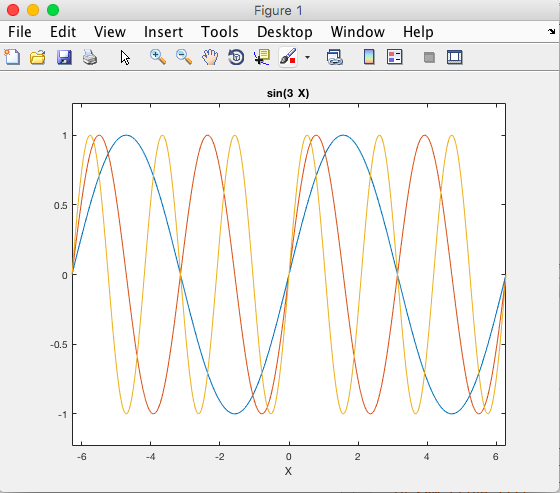
\includegraphics[scale=0.3]{images/fig5.png}
\end{center}
\end{frame}

\begin{frame}{Cálculo: Introducción a la diferenciación}
Se considera un auto de carreras cuya ecuación de posición es:
\begin{equation*}
d=20+20*sen(\frac{\pi *(t-10))}{20})
\end{equation*}
\begin{center}
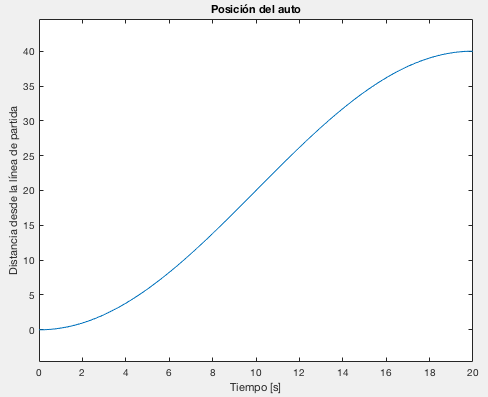
\includegraphics[scale=0.3]{images/fig6.png}
\end{center}
\end{frame}

\begin{frame}{Cálculo: Introducción a la diferenciación}
Sabiendo que la velocidad es la derivada de la posición y utilizando la función \textbf{diff}
\begin{exampleblock}{Comando}
Ver comando: diff()
\end{exampleblock}
\begin{center}
Curva de velocidad
\end{center}
\begin{center}
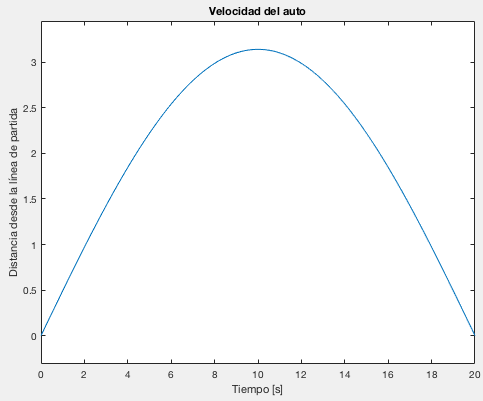
\includegraphics[scale=0.3]{images/fig7.png}
\end{center}
\end{frame}

\begin{frame}{Cálculo: Introducción a la diferenciación}
Sabiendo que la aceleración es la derivada de la velocidad y utilizando la función \textbf{diff}
\begin{exampleblock}{Comando}
Ver comando: diff()
\end{exampleblock}
\begin{center}
Curva de aceleración
\end{center}
\begin{center}
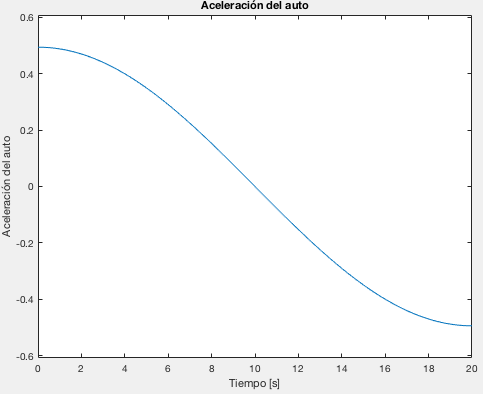
\includegraphics[scale=0.3]{images/fig8.png}
\end{center}
\end{frame}

\begin{frame}{Cálculo: Introducción a la diferenciación}
\textbf{Funciones de diferenciación simbólica:}
\begin{table}[]
\centering
\begin{tabular}{|c|c|}
\hline
diff(f)       & Derivada de f respecto a la variable independiente     \\ \hline
diff(f,'t')   & Derivada de f respecto a la variable t                 \\ \hline
diff(f,n)     & Derivada n-ésima de f respecto a la variable independeinte \\ \hline
diff(f,'t',n) & Derivada n-ésima de f respecto a la variable t             \\ \hline
\end{tabular}
\end{table}
\end{frame}

\begin{frame}{Ejercicio práctico 20}
\begin{enumerate}
\item Encuentre la primera derivada con respecto a x de las siguientes expresiones:
\begin{enumerate}
\item $x^2+x+1$
\item $sen(x)$
\end{enumerate}
\item Encuentre la primera derivada parcial con respecto a x de las siguientes expresiones:
\begin{enumerate}
\item $x^{0.5 }-3*y$
\item $3*x+4*y-3*x*y$
\end{enumerate}
\item Encuentre la segunda derivada con respecto a x para cada una de las expresiones del problema 1 y 2.
\item Encuentre la primera derivada con respecto a y para las siguientes expresiones:
\begin{enumerate}
\item $y-1$
\item $a*y+b*x+c*z$
\end{enumerate}
\end{enumerate}
\end{frame}

\begin{frame}{Cálculo: Introducción a la integración}
Dada la curva de aceleración se procede a calcular la velocidad integrando la misma. 
\begin{exampleblock}{Comando}
Ver comando: int()
\end{exampleblock}
\begin{center}
Curva de velocidad
\end{center}
\begin{center}
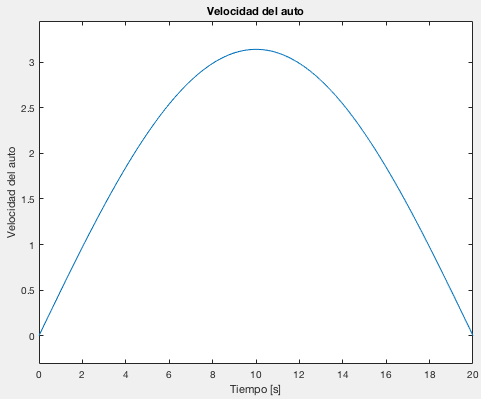
\includegraphics[scale=0.3]{images/fig9.png}
\end{center}
\end{frame}

\begin{frame}{Cálculo: Introducción a la integración}
\textbf{Cálculo de integral definida:}
\begin{table}[]
\centering
\begin{tabular}{|c|c|}
\hline
int(f)     & Integral de f respecto a la variable independiente                                                                      \\ \hline
int(f,'t') & Integral de f respecto a la variable t                                                                                  \\ \hline
int(f,a,b) & \begin{tabular}[c]{@{}c@{}}Integral respecto a la variable independiente de f entre a y b\end{tabular} \\ \hline
\end{tabular}
\end{table}
\end{frame}

\begin{frame}{Ejercicio práctico 21}
\begin{enumerate}
\item Integre las siguientes expresiones con respecto a x:
\begin{enumerate}
\item $x^2+x+1$
\item $tan(X)$
\end{enumerate}
\item Integre las siguientes expresiones con respecto a x:
\begin{enumerate}
\item $x^{0.5 }-3*y$
\item $3*x+4*y-3*x*y$
\end{enumerate}
\item Realice una integración doble con respecto a x para cada una de las expresiones de los problemas 1 y 2.
\item Integre las siguientes expresiones con respecto a y:
\begin{enumerate}
\item $y-1$
\item $a*y+b*x+c*z$
\end{enumerate}
\end{enumerate}
\end{frame}

\begin{frame}{Ejercicio práctico 21}
\begin{center}

\includegraphics[scale=0.4]{images/img41.png}
\end{center}
\end{frame}

\end{document}
